% Mooers2021TemplatesNotes

\subsubsection*{Summary}
PyMOL commands offer precise control over the visualization of molecular models, making PyMOL a favored tool for creating images of protein structures for publications and presentations. However, many users struggle to remember these commands due to infrequent use, complicating writing new scripts. 
One practical approach to address this issue is using code fragments as templates for different parts of the task. 
These fragments can be accessed from a library while coding in text editors like Visual Studio Code, Vim, and Emacs.


To facilitate this, we developed a library of PyMOL code templates, known as pymolsnips, which simplifies the process of writing PyMOL scripts. 
Pymolsnips is available on GitHub in formats compatible with 18 popular text editors, supporting Mac, Windows, and Linux operating systems. 
The GitHub repository also includes animations to guide users through the installation process for each text editor. 
This library will significantly enhance the productivity of PyMOL users when scripting.


\subsubsection*{Context in Molecular Graphics and Human-Computer Interaction}
\begin{wrapfigure}{l}{0.35\textwidth} % Example figure with text wrapping around it
\vspace{-10pt}
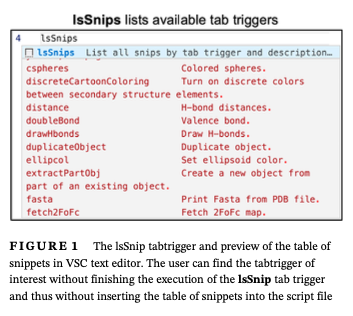
\includegraphics[scale=0.4]{imagesBlaine/Mooers2021TemplatesFig1.png}
\caption{\footnotesize Text wrapped image }
\vspace{-10pt}
\label{fig:preview}
\end{wrapfigure}

Tools like PyMOL and libraries like pymolsnips play a crucial role in the broader context of molecular graphics and human-computer interaction. 
Molecular graphics software allows scientists to visualize complex molecular structures, aiding in the understanding and communicating biochemical processes. 
The ability to precisely control these visualizations is essential for producing high-quality images for research and educational purposes.


Human-computer interaction (HCI) principles are integral to the design of these tools, ensuring they are user-friendly and accessible.
Visual Studio Code provide excellent usr interface to snippets (See Fig \ref{fig:preview}). 
By providing code snippets and templates, pymolsnips enhances the usability of PyMOL, making it easier for users to create and modify scripts without needing to recall specific commands. 
This approach aligns with HCI goals of improving efficiency and reducing cognitive load, ultimately fostering a more productive and intuitive user experience.

\subsubsection*{Snippet interfaces in Text Editors}

Pymolsnips can be used at all skill levels (Table \ref{tab:skilllevel}).
PyMOL users can be divided into five levels of skill \cite{Dreyfus1980AFiveStageModelOfTheMentalActivitiesInvolvedInDirectedSkillAcquisition}. 
Beginner users may represent ~40\% of PyMOL users (Table 1). 
Their use of PyMOL is generally limited to viewing and comparing structures.
Beginner users are not yet willing to invest in learning the commands of the PyMOL macro language. 
They prefer the intuitive nature of the PyMOL GUI and its pulldown menus. 

\begin{table}[h]
\begin{center}
\caption{Tools by target skill level.}
\begin{tabular}{l c c c c}
\toprule
\multicolumn{1}{l}{\bf{Skill level}} & {\bf{Shortcuts}} & {\bf{Snippets}} & {\bf{Polyglot docs}} & {\bf{Quizzes}}\\
\midrule
Beginner        &  \checkmark  &           &             &  \checkmark  \\
Adv. Beginner   &  \checkmark & \checkmark &             &   \checkmark  \\
Competent       &  \checkmark & \checkmark &  \checkmark &   \checkmark  \\
Proficient.     &  \checkmark & \checkmark &  \checkmark &   \checkmark   \\
Expert          &  \checkmark & \checkmark &  \checkmark &   \checkmark   \\
\hline 
\end{tabular}
\end{center}
\end{table}

Advanced beginners (~30\% of users) are able to navigate the GUI quickly. 
They also use simple commands like the ``fetch'' command to retrieve coordinate files from the Protein Data Bank. 
They may make images of global views and structure superpositions. 
They also make simple close-up views of protein-ligand interactions and subunit-subunit interfaces. 
They rely on session files to save work in progress. 
Competent users (~20\% of users) use scripts to assemble images for publication.
Proficient users (~9\% of users) know most of the frequently used parameters and are willing to invest time in learning new commands. 
They have been using text editors for years but may not have discovered the power of snippet libraries. 

The expert users (~1\%) understand the PyMOL macro language syntax and remember many of the commands. 
They extend the capability of PyMOL by importing functions from modules outside of PyMOL.
They may even be involved in the development of new plugins. 
They are likely expert users of one or more text editors. 
They would welcome a snippet library and the shortcuts. 
The tools developed in this proposal will benefit users at all levels of expertise and help them to move to higher levels of expertise (Table 1).


% % You have to tweak the textwidth to move the caption to the right to align with the table.
% \begin{wraptable}{r}{0.60\textwidth} % Example table with text wrapping around it
% \caption{Tools by target skill level.}
% \begin{center}
% \vspace{-20pt}
% \begin{threeparttable}
% \begin{tabular}{l c c c c}
% \toprule
% \multicolumn{1}{l}{\bf{Skill level}} & {\bf{Shortcuts}} & {\bf{Snippets}} & {\bf{Polyglot docs}} & {\bf{Quizzes}}\\
% \midrule
% Beginner        &  \checkmark  &           &             &  \checkmark  \\
% Adv. Beginner   &  \checkmark & \checkmark &             &   \checkmark  \\
% Competent       &  \checkmark & \checkmark &  \checkmark &   \checkmark  \\
% Proficient.     &  \checkmark & \checkmark &  \checkmark &   \checkmark   \\
% Expert          &  \checkmark & \checkmark &  \checkmark &   \checkmark   \\
% \hline
% \end{tabular}
% \end{threeparttable}
% %\footnotesize\textsuperscript{a}{All participants clowns.}
% \vspace{-10pt}
% \end{center}
% \label{tab:skilllevel}
% \end{wraptable}

